\section{Design}
I vores design har vi vægtet at hver class vi implementere har ét ansvar. Det vil sige at det ikke nødvendigvis er den class som indeholder informationen som bearbejder den. At følge dette princip har den svaghed at kommunikationskæden vil blive længere en den behøver hvilket ultimativt vil lede til at vores program vil køre langsommere. Tilgengæld vil vores kodebase være nemmere at maintain da det vil blive tydeligt hvor hvilken opgave bliver udført og det vil derfor også blive nemmere at identificere hvor bugs opstår. Vi har også fulgt princip om at hver klasse selv udfører sit arbejde og vi har derfor ikke klasser som er afhængige af andre klassers metoder, men vi har klasser som er afhængige af andre klasser.\\
Vi kan bekræfte det ovenstående ud fra vores traceability matrix som netop mapper hvert af vores koncepter med en implementeret class, hvilket betyder at hver af vores klasser kun har ét ansvar. Mængden af klasser kan være en indikation på at kommunikationskæden er lang, mens det at der ikke er nogen koncepter som mapper til mere end en klasse fortæller os at arbejdsbyrden er jævnt fordelt.\\

\begin{table}[]
\centering
\caption{My caption}
\label{my-label}
\begin{tabular}{|l|l|l|l|l|l|l|l|l|}
\hline
              & Program & LL & FR & LCl & Game & LCr & EC & LK \\\hline
Program       & x       &             &            &       &      &              &               &             \\\hline
LevelLoader   &         & x           &            &       &      &              &               &             \\\hline
FileReader    &         &             & x          &       &      &              &               &             \\\hline
Level class        &         &             &            & x     &      &              &               &             \\\hline
Game          &         &             &            &       & x    &              &               &             \\\hline
LevelCreator  &         &             &            &       &      & x            &               &             \\\hline
EntityCreator &         &             &            &       &      &              & x             &             \\\hline
LevelKeeper   &         &             &            &       &      &              &               & x\\\hline
\end{tabular}
\end{table}

Ud fra vores sequence diagram, som ses på figur \ref{seqDig}, kan det ses at vores design arbejder af to omgange. LevelLoader beder FileReader om at læse en levelfil hvorefter at FileReader benytter informationerne fra levelfilen til kalde konstruktoren i Level for at lave et nyt level objekt som bliver givet tilbage til LevelLoader. I LevelLoader hentes der en instans af LevelsKeeper som bruges til at gemme level objektet. Dette loop bliver gentaget for alle de levelfiler som er specificeret i LevelLoader hvilket udgør den første del af vores design. LevelLoader bliver brugt ude i Program hvilket sørger for at alle levels i spillet er loadet inden brugeren får givet nogen form for kontrol. Dette vil kunne give problemer med hastigheden af opstart af spillet hvis der skal loades en meget stor mængde af levels, mens at det vil sikre en hurtig transition mellem levels. Da vi ikke forventer der skal loades store mængder af levels, så vil vi placere en lille ventetid i opstarten af programmet og dermed opnå et hurtigt skift mellem levels. \\
Den anden del bliver udgjort af Game som beder LevelCreator om en EntityContainer for de blokke som skal udgøre det level som skal tegnes. LevelCreator indeholder også en instans af LevelsKeeper som nu benyttes til at hente et specifikt level som er blevet gemt. LevelCreator benytter oplysningerne i det hentede level objekt til at bede EntityCreator om at lave en ny entity som skal udgøre en blok i et level. LevelCreator gemmer denne entity i en EntityContainer, og når alle blokke er blevet bygget returneres EntityContaineren og Game kan derefter render den.\\
\begin{figure}
  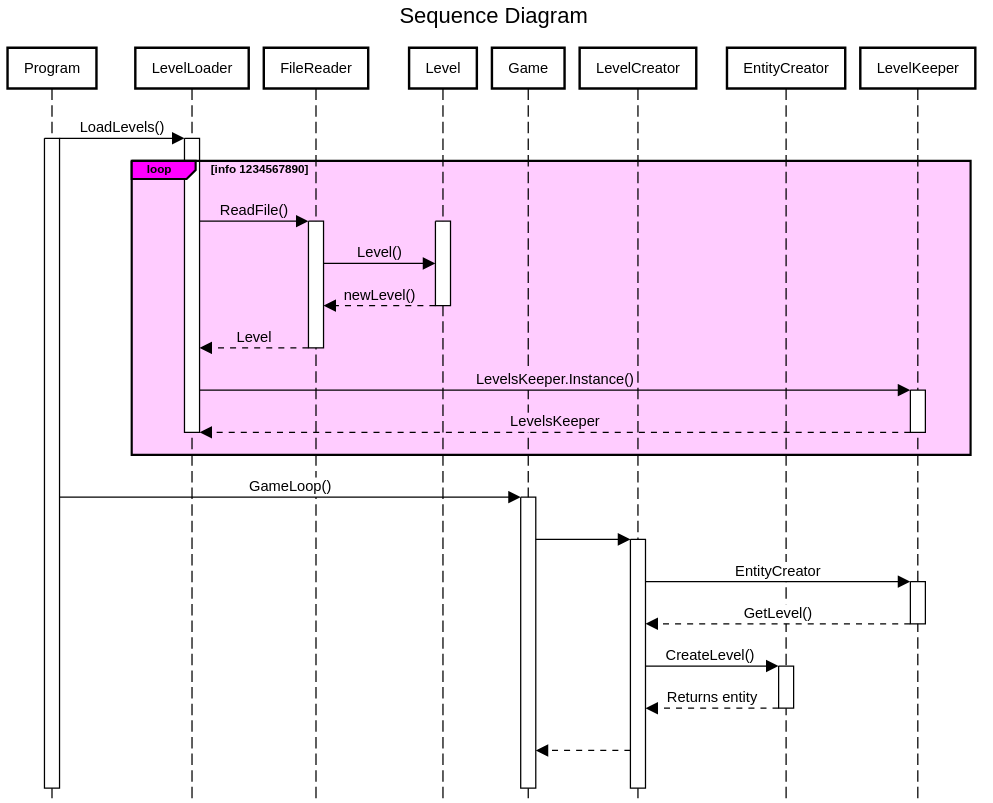
\includegraphics[width=\linewidth]{latex/Images/SequenceDiagram.png}
  \caption{Sequence diagram}
  \label{seqDig}
\end{figure}
